\begin{figure*}[H]
    \centering

    \subfloat[\Sh]{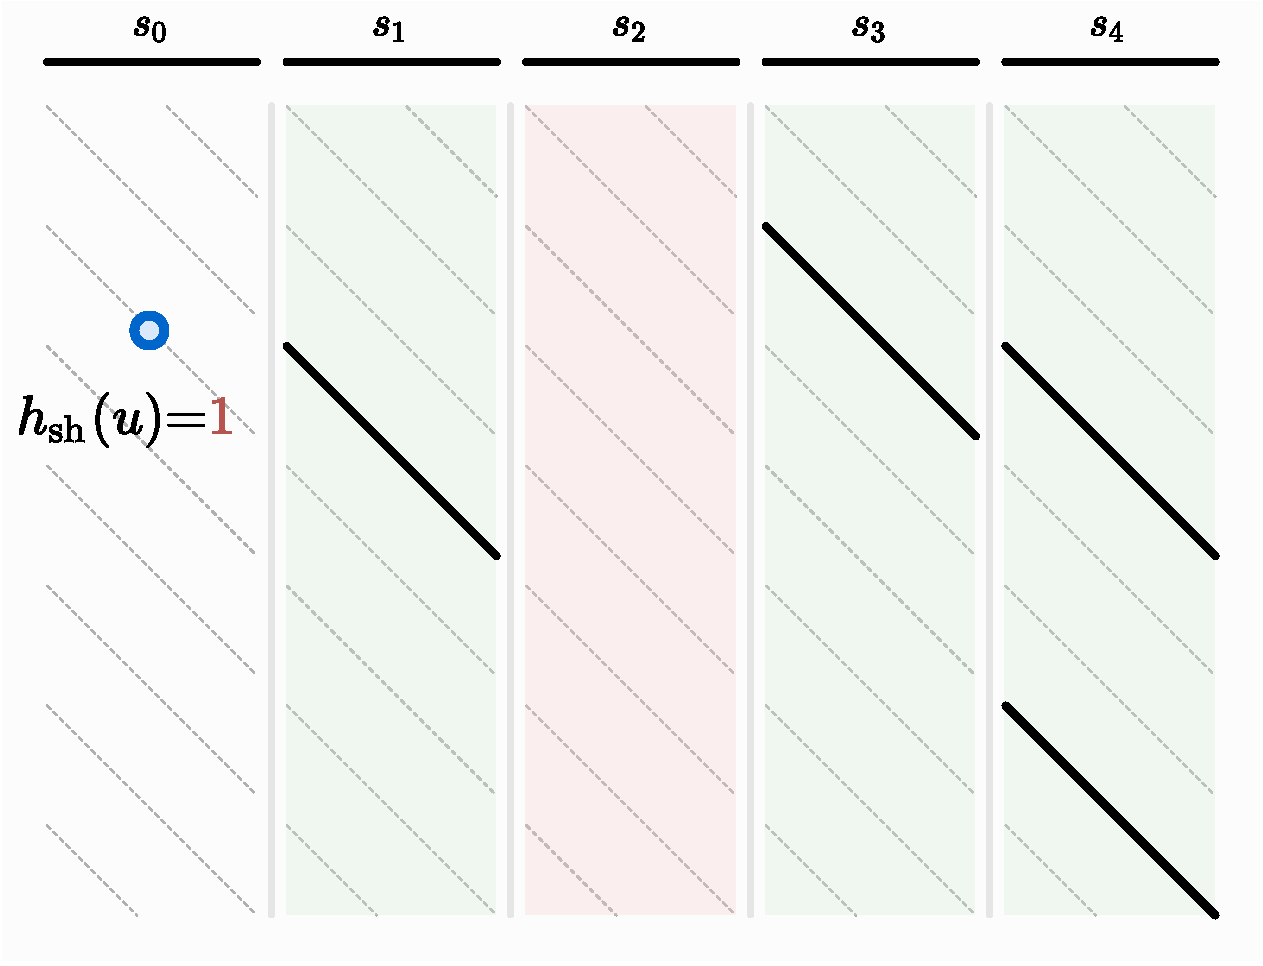
\includegraphics[width=0.24\linewidth]{imgs/heuristic-diagrams/sh.pdf}\label{fig:sh}}
    \hfill
    \subfloat[\Csh]{
\includegraphics[width=0.24\linewidth]{imgs/heuristic-diagrams/csh.pdf}\label{fig:csh}}
    \hfill
    \subfloat[\Gch]{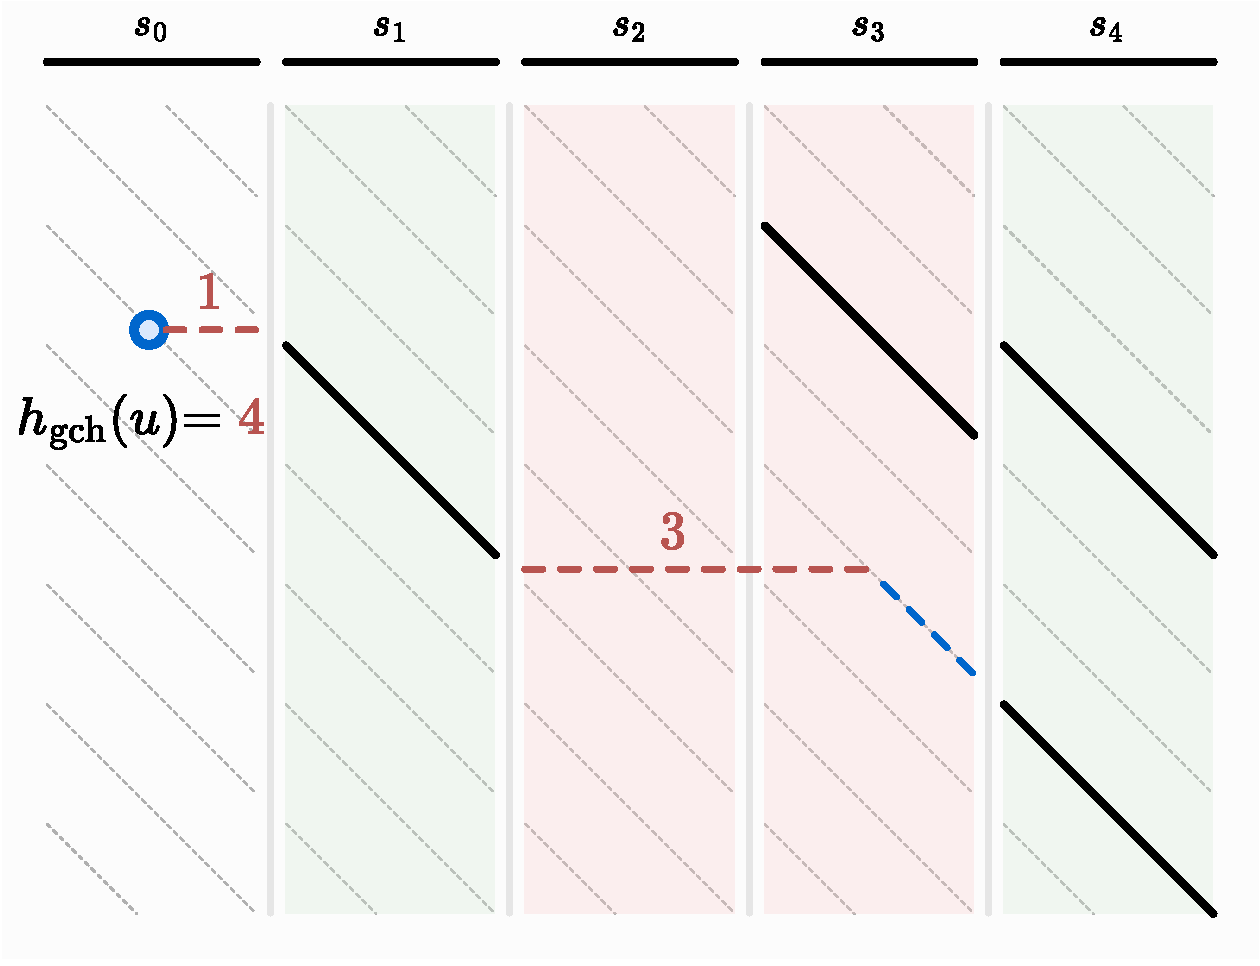
\includegraphics[width=0.24\linewidth]{imgs/heuristic-diagrams/gch.pdf}\label{fig:gch}}
    \hfill
    \subfloat[\CSH + match pruning]{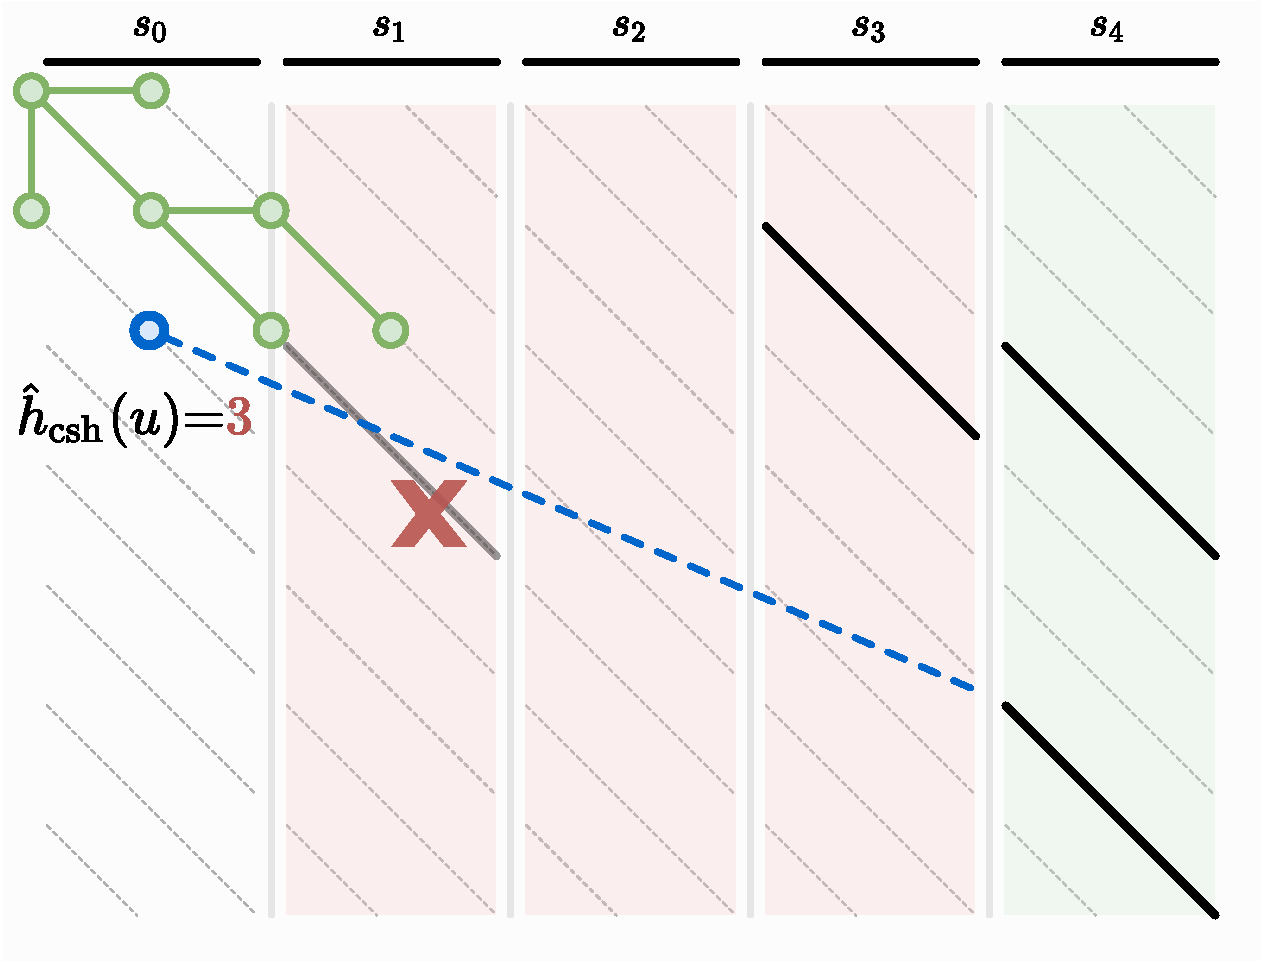
\includegraphics[width=0.24\linewidth]{imgs/heuristic-diagrams/pruning.pdf}\label{fig:pruning}}

    \caption[Family of chaining seed heuristics]{\textbf{Demonstration of \sh, \csh, \gch, and match pruning.}
      Sequence $A$ is split into $5$ seeds (horizontal black segments \seed) on
      top. Each seed is exactly matched in $B$ (diagonal black segments \match).
      The heuristic is evaluated at state $u$ (blue circles \bluecircle), based
      on the $4$ remaining seeds. The heuristic value is based on a maximal
      chain of matches (green columns \greencolumn\ for seeds with
      matches; red columns \redcolumn\ otherwise). Dashed lines denote chaining
      of matches.
      %
      \protect\subref{fig:sh} The \sh $\hsh(u) {=} 1$ is the number of remaining
      seeds that do not have matches (only $s_2$).
      %
      \protect\subref{fig:csh} The \csh $\hcsh(u) {=} 2$ is the number of
      remaining seeds without a match ($s_2$ and $s_3$) on a path going only
      down and to the right containing a maximal number of matches.
      %
      \protect\subref{fig:gch} The \gch $\hgch(u) {=} 4$ is minimal cost of a
      chain, where the cost of joining two matches is the maximum of the number
      of not matched seeds and the gap cost between them. Red dashed lines
      denote gap costs.
      %
      \protect\subref{fig:pruning} Once the start or end of a match is expanded
      (green circles \greencircle), the match is \emph{pruned} (red cross
      \cross), and future computations of the heuristic ignore it. $s_1$ is
      removed from the maximum chain of matches starting at $u$ so $\hcshS(u)$
      increases by $1$.}
    \label{fig:heuristics}
\end{figure*}
